% =============================================================
% บทที่ 2 - ทฤษฎีและงานวิจัยที่เกี่ยวข้อง
% หัวข้อ: การวิเคราะห์และทำนายผลการแข่งขันฟุตบอลลีกยุโรปด้วยกระบวนการวิทยาการข้อมูล
%        เพื่อการประเมินมูลค่าการเดิมพัน
% =============================================================

% -----------------------------------------------------------
\section{ทฤษฎีที่เกี่ยวข้อง}
% -----------------------------------------------------------

\subsection{กระบวนการวิทยาการข้อมูลและการจัดทำท่อส่งข้อมูล (Data Science \& Pipeline Process)}

กระบวนการวิทยาการข้อมูลเป็นกรอบการทำงานเชิงระบบที่นำข้อมูลขนาดใหญ่มาประมวลผลและวิเคราะห์ เพื่อค้นหารูปแบบหรือสร้างคุณประโยชน์ ในโครงงานนี้ได้ประยุกต์ใช้กระบวนการ 5 ขั้นตอน ร่วมกับการออกแบบท่อส่งข้อมูลแบบโมดูลาร์ (Modular Data Pipeline) ได้แก่

\begin{enumerate}[label=\arabic*)]
    \item \textbf{การกำหนดวัตถุประสงค์และคำถามวิจัย (Question Refinement):} กำหนดโจทย์การทำนายผลการแข่งขันฟุตบอลออกเป็น 3 รูปแบบ ได้แก่ ทีมเจ้าบ้านชนะ (Home Win: H), เสมอ (Draw: D) และทีมเยือนชนะ (Away Win: A) เพื่อนำไปประเมินความคุ้มค่าในการเดิมพันเชิงสถิติ
    \item \textbf{การเก็บรวบรวมข้อมูล (Data Collection):} การสร้างระบบดึงข้อมูลอัตโนมัติ เพื่อรวบรวมตารางการแข่งขัน ผลประตู ค่า xG และสถิติรายบุคคลจาก Understat, ปฏิทินการแข่งขันและแผนการเล่นจาก Transfermarkt รวมถึงสถิติผลการแข่งขันย้อนหลังและราคาอัตราต่อรอง (Betting Odds) จาก Football-Data.co.uk \cite{footballdata, transfermarkt2024, understat2024}
    \item \textbf{การตรวจสอบ ทำความสะอาด และสร้างตัวแปร (Data Validation \& Feature Engineering):} การตรวจสอบคุณภาพข้อมูลผ่านสัญญาข้อมูล (Data Contracts / Pandera) การจัดการค่าที่ขาดหาย การจับคู่ชื่อสโมสร (Entity Resolution) และการสร้างตัวแปรก่อนการแข่งขัน เช่น คะแนน Elo, ดัชนีความเหนื่อยล้า, ความหนาแน่นของตารางแข่งขัน และฟอร์มของผู้เล่นตัวจริง 11 คนแรก
    \item \textbf{การสร้างและประเมินแบบจำลอง (Model Building \& Evaluation):} การพัฒนาแบบจำลองเพื่อทำนายความน่าจะเป็นที่แท้จริงของผลการแข่งขัน และประเมินประสิทธิภาพด้วยตัวชี้วัด Log Loss, Ranked Probability Score (RPS) และ Accuracy \cite{scikit-learn}
    \item \textbf{การสรุป วิเคราะห์ตลาด และการจำลองเดิมพัน (Market Analysis \& Backtesting):} การวิเคราะห์ราคาต่อรองเพื่อหาโอกาสการเดิมพันที่มีมูลค่า (Value Betting) การประเมินผลกำไร/ขาดทุนสะสม (ROI) ด้วยกลยุทธ์การวางเงินทุนรูปแบบต่าง ๆ และการนำเสนอระดับความสำคัญของตัวแปรทำนาย (Feature Importance)
\end{enumerate}

\subsection{ระบบวัดระดับความแข็งแกร่ง (Elo Rating System)}

ระบบคะแนน Elo เป็นวิธีทางสถิติที่ใช้คำนวณระดับทักษะความแข็งแกร่งของทีมแข่งขัน คะแนนจะถูกปรับเปลี่ยนตามผลการแข่งขันจริงและระดับความแข็งแกร่งของคู่แข่ง โดยทีมที่ชนะทีมที่มีคะแนนสูงกว่าจะได้คะแนนเพิ่มขึ้นมากกว่าการชนะทีมที่อ่อนกว่า \cite{hvattum2010using} สำหรับฟุตบอล การปรับคะแนนสามารถถ่วงน้ำหนักตามผลต่างประตูของการแข่งขันได้ เพื่อให้ชัยชนะที่ขาดลอยส่งผลต่อคะแนนมากกว่าชัยชนะเฉียดฉิว ในโครงงานนี้ได้มีการคำนวณค่า Elo Rating ของแต่ละสโมสรอย่างต่อเนื่องตามลำดับเวลา (Time-series) ดังแสดงในรูปที่ \ref{fig:elo_concept} และนำผลต่างคะแนน Elo (Elo Difference) ระหว่างทีมเจ้าบ้านและทีมเยือน ซึ่งใช้ค่าก่อนเริ่มการแข่งขันเท่านั้น มาใช้เป็นตัวแปรสำคัญในการสะท้อนความได้เปรียบเชิงศักยภาพของทีม

\begin{figure}[H]
    \centering
    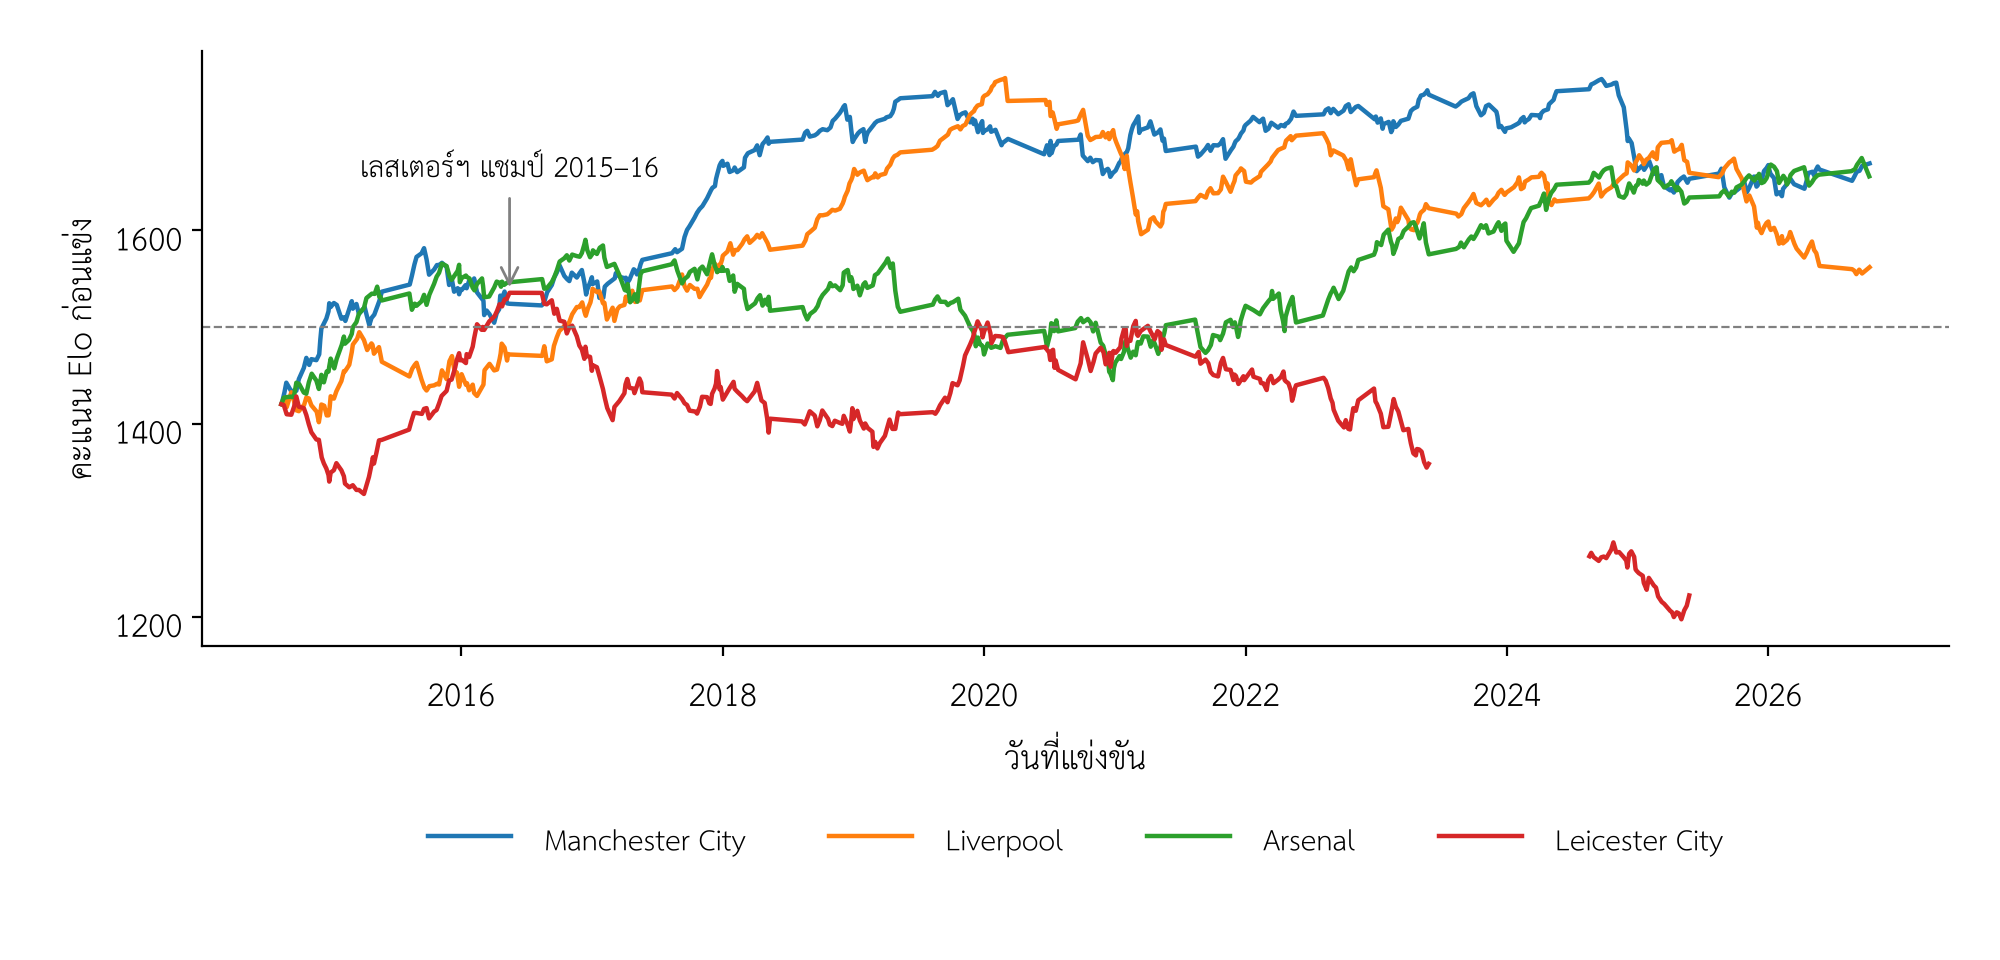
\includegraphics[width=\textwidth]{images/elo_history.png}
    \caption{คะแนน Elo ก่อนแข่งของ 4 สโมสรพรีเมียร์ลีกที่คำนวณในโครงงานนี้ (เส้นประคือคะแนนเริ่มต้น 1500 ช่วงที่เส้นขาดคือฤดูกาลที่สโมสรไม่ได้อยู่ใน 5 ลีกใหญ่)}
    \label{fig:elo_concept}
\end{figure}

\subsection{ค่าความคาดหวังในการทำประตู (Expected Goals: xG)}

ค่า xG เป็นตัวชี้วัดเชิงสถิติขั้นสูงที่ใช้ประเมินคุณภาพของโอกาสในการยิงประตู โดยคำนวณความน่าจะเป็นที่ลูกยิงแต่ละครั้งจะกลายเป็นประตู (มีค่าระหว่าง 0 ถึง 1) ขึ้นอยู่กับตำแหน่งการยิง มุมในการยิง ประเภทการส่งบอล และบริบทของเกม ดังแสดงตัวอย่างในรูปที่ \ref{fig:xg_concept} ซึ่ง Liverpool ยิง 18 ครั้ง รวม xG 3.70 ขณะที่ Manchester City ยิง 8 ครั้ง รวม xG เพียง 0.75 ค่า xG ช่วยให้มองเห็นประสิทธิภาพเกมรุกที่แท้จริง ซึ่งสะท้อนฟอร์มการเล่นได้ดีกว่าผลสกอร์แพ้-ชนะแบบดั้งเดิม \cite{understat2024} ในโครงงานนี้ ค่า xG และค่า xA (Expected Assists) รายบุคคลถูกนำมาสรุปเป็นฟอร์มของผู้เล่นตัวจริงแต่ละคน ในรูปอัตราต่อ 90 นาที โดยใช้เฉพาะการแข่งขันก่อนนัดปัจจุบัน

\begin{figure}[H]
    \centering
    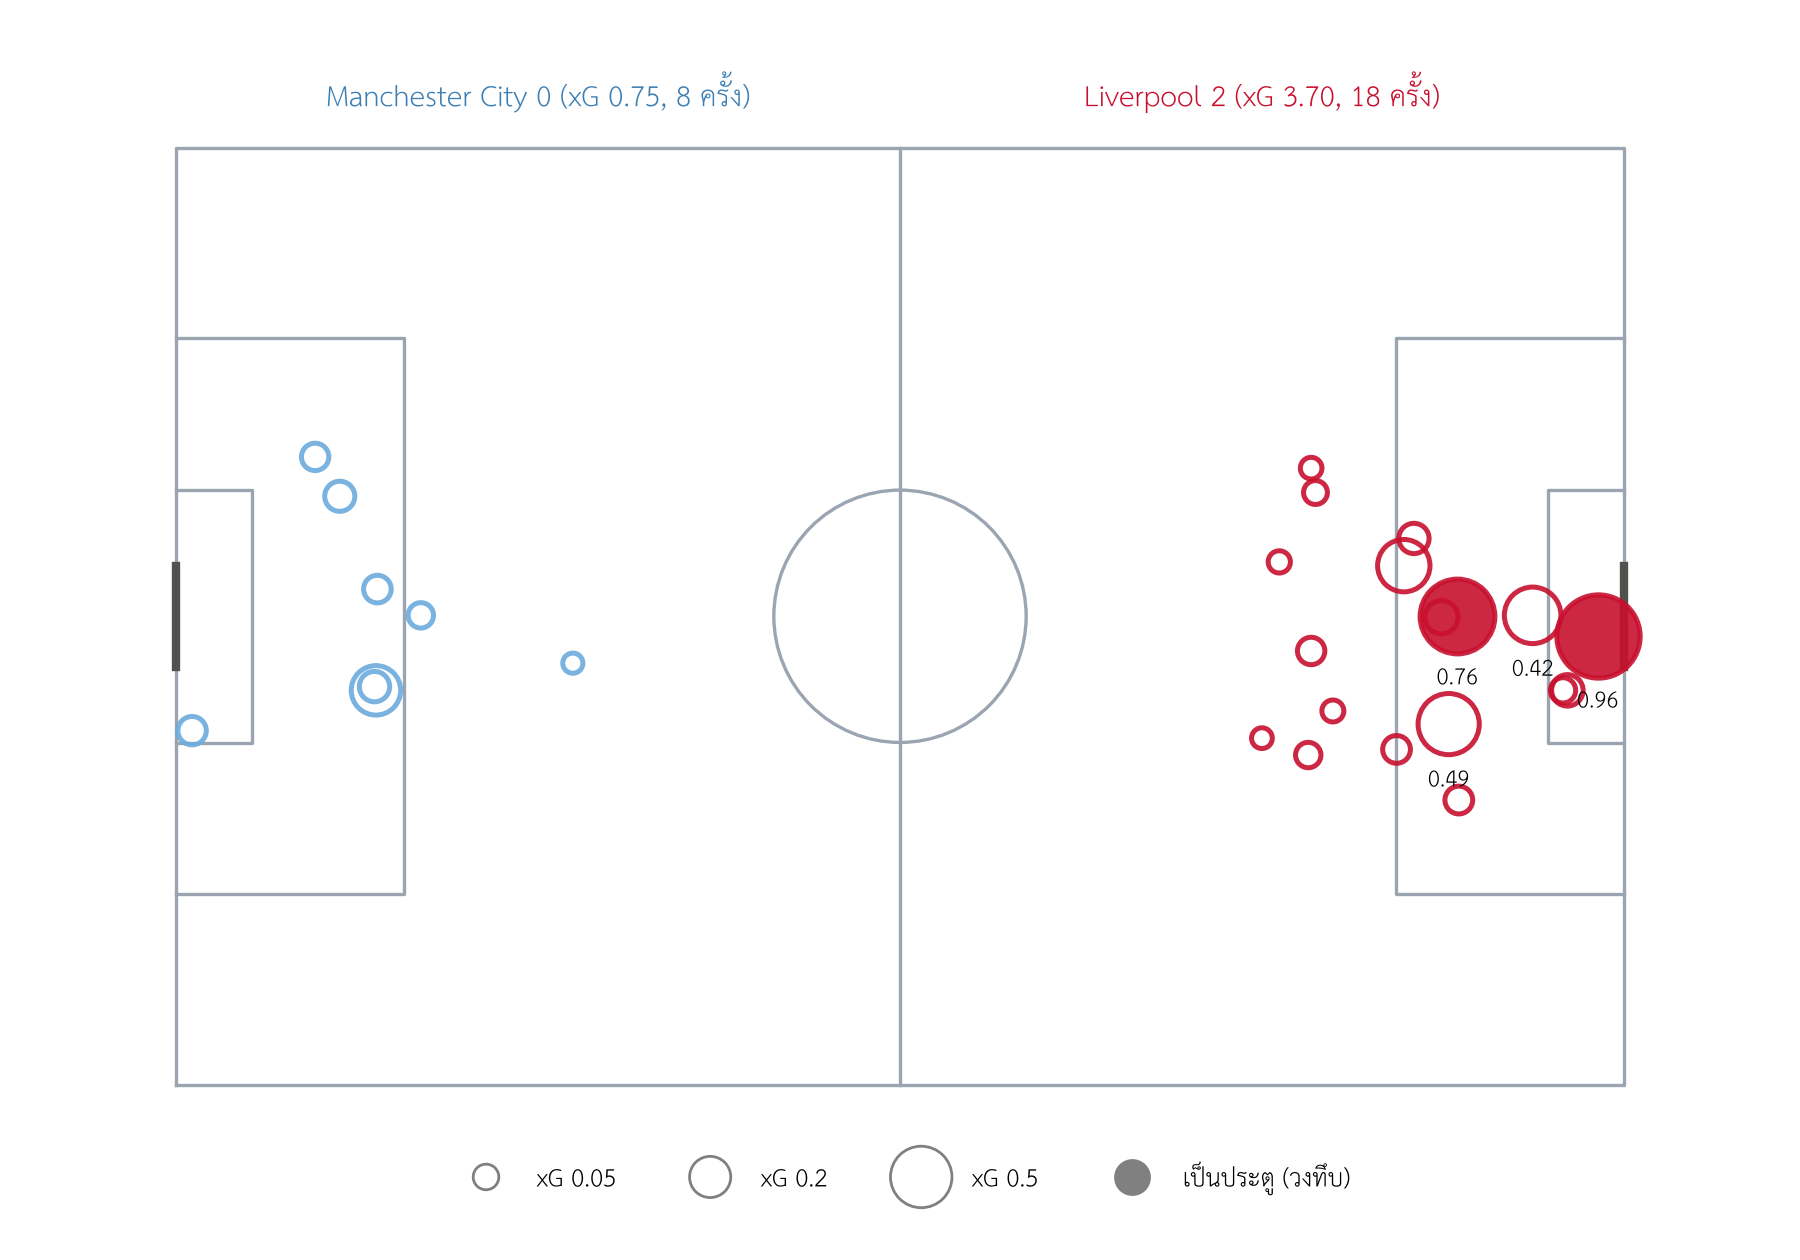
\includegraphics[width=0.9\textwidth]{images/xg_shot_map.png}
    \caption[ตำแหน่งการยิงและค่า xG ของแต่ละลูกในนัด Liverpool 2--0 Manchester City]{ตำแหน่งการยิงและค่า xG ของแต่ละลูกในนัด Liverpool 2--0 Manchester City (1 ธันวาคม 2024) ขนาดวงตามค่า xG วงทึบคือลูกที่เป็นประตู (ข้อมูลจาก Understat \cite{understat2024})}
    \label{fig:xg_concept}
\end{figure}

\subsection{ดัชนีความเหนื่อยล้าและความหนาแน่นของตารางแข่ง (Fatigue Metric \& Schedule Congestion)}

ระยะเวลาพักผ่อนระหว่างแมตช์การแข่งขันส่งผลต่อสภาพร่างกายและประสิทธิภาพการเล่นของนักเตะ ในโครงงานนี้จึงสร้างตัวแปรที่เกี่ยวข้องกับภาระการเล่นเป็น 2 ระดับ ดังแสดงตัวอย่างแนวคิดในรูปที่ \ref{fig:fatigue_concept}

\begin{enumerate}[label=\arabic*)]
    \item \textbf{ระดับผู้เล่น:} คำนวณคะแนนความเหนื่อยล้า (Fatigue Score) ช่วง 0--100 จากนาทีที่ลงเล่นใน 7 และ 28 วันก่อนหน้า (ภาระงานระยะสั้นเทียบกับระยะยาว) และความสั้นของระยะพัก แล้วสรุปเป็นค่าเฉลี่ยของผู้เล่นตัวจริงแต่ละฝั่ง
    \item \textbf{ระดับทีม:} คำนวณจากปฏิทินการแข่งขันทุกรายการ ได้แก่ จำนวนวันพักนับจากนัดก่อนหน้า จำนวนนัดใน 7 และ 14 วันที่ผ่านมา จำนวนนัดที่ไม่ใช่ลีกใน 14 วัน และการเดินทางไปเยือนในศึกยุโรปในนัดก่อนหน้า
\end{enumerate}

\begin{figure}[H]
    \centering
    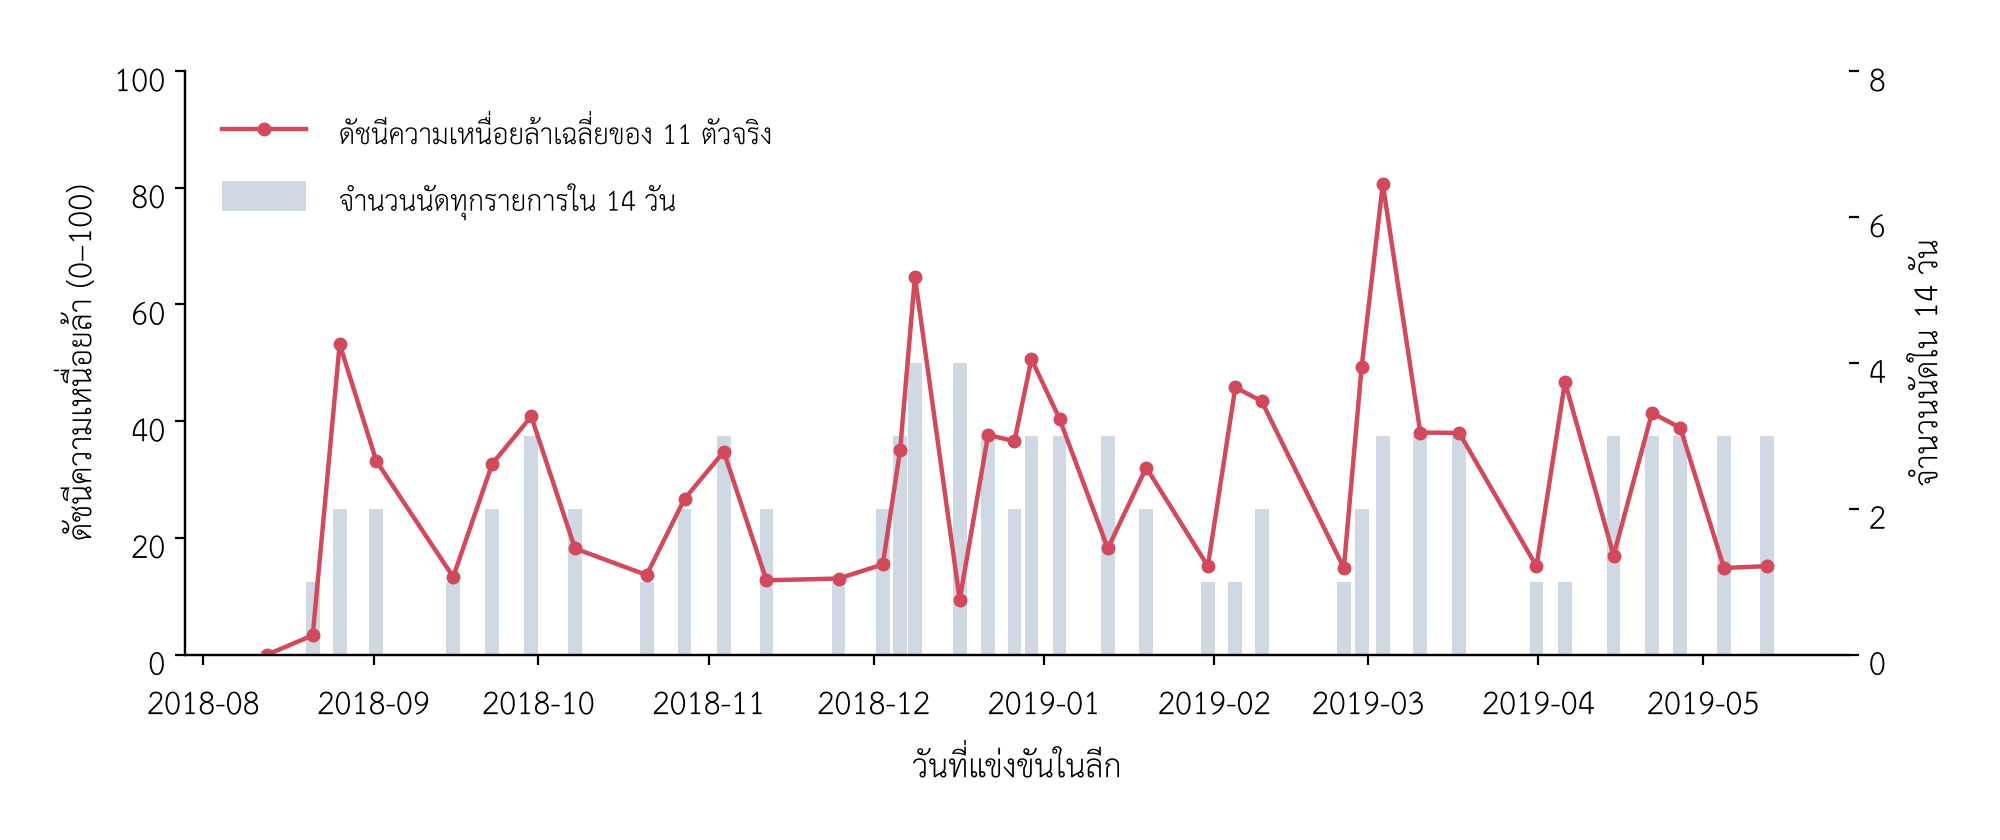
\includegraphics[width=\textwidth]{images/fatigue_season.png}
    \caption{ดัชนีความเหนื่อยล้าเฉลี่ยของผู้เล่นตัวจริงและจำนวนนัดทุกรายการใน 14 วันก่อนแต่ละนัดในลีกของ Liverpool ฤดูกาล 2018--2019}
    \label{fig:fatigue_concept}
\end{figure}

\subsection{อัตราต่อรองของเจ้ามือรับพนันและการเดิมพันที่มีมูลค่า (Betting Odds \& Value Betting)}

ราคาอัตราต่อรองจากเจ้ามือรับพนัน (Bookmakers) สามารถแปลงเป็นค่าความน่าจะเป็นโดยนัย (Implied Probability) ได้ โดยคำนวณจากส่วนกลับของราคาต่อรอง เช่น อัตราจ่าย $O$ จะมีความน่าจะเป็นโดยนัยเท่ากับ $1/O$ อย่างไรก็ตาม ผลรวมความน่าจะเป็นของทุกทางเลือก (Home/Draw/Away) มักจะเกินร้อยละ 100 เนื่องจากถูกบวกส่วนต่างกำไรของเจ้ามือ (Overround / Vig)

การวิเคราะห์เพื่อการเดิมพันจะใช้แบบจำลองคำนวณ \textbf{ความน่าจะเป็นที่แท้จริง (Model Probability: $P$)} แล้วนำไปเปรียบเทียบกับราคาต่อรองในตลาด หากราคาต่อรองในตลาดให้ค่าสูงกว่าความน่าจะเป็นของแบบจำลอง จะถือว่าเกิด \textbf{การเดิมพันที่มีมูลค่าคาดหมายเป็นบวก (Positive Expected Value: +EV / Value Bet)} โดยค่าความคาดหมายคำนวณได้จาก:
\begin{equation}
    EV = (P \times O) - 1
\end{equation}
หากค่า $EV > 0$ แสดงว่าการวางเดิมพันในตัวเลือกนั้นมีความคุ้มค่าทางสถิติในระยะยาว

\subsection{กลยุทธ์การบริหารเงินทุนและการทดสอบย้อนหลัง (Staking Strategies \& Backtesting)}

ในการประเมินผลตอบแทนทางการเงิน การทำนายผลถูกต้องเพียงอย่างเดียวไม่เพียงพอ แต่ต้องอาศัยกลยุทธ์การจัดสรรเงินทุน (Staking Strategy) ที่เหมาะสม เพื่อป้องกันความเสี่ยงจากการหมดตัว (Risk of Ruin) โครงงานนี้ทดสอบแผนการวางเงิน 5 แบบ แบ่งเป็น 3 กลุ่ม ได้แก่:
\begin{enumerate}[label=\arabic*)]
    \item \textbf{การวางเงินคงที่ (Fixed Staking):} กำหนดจำนวนเงินวางเดิมพันเป็นจำนวนเงินที่แน่นอนเท่ากันทุกครั้ง
    \item \textbf{สูตรการวางเงินแบบเคลลี (Kelly Criterion):} คำนวณสัดส่วนเงินทุนที่ควรวางเดิมพัน ($f^*$) ตามระดับความคุ้มค่าและอัตราต่อรอง:
    \begin{equation}
        f^* = \frac{P \cdot O - 1}{O - 1}
    \end{equation}
    พร้อมทั้งทดสอบสัดส่วนเคลลีแบบย่อย (Fractional Kelly ได้แก่ Half Kelly และ Quarter Kelly) เพื่อลดความผันผวนของเงินทุน
    \item \textbf{Martingale:} เพิ่มเงินเดิมพันเป็น 2 เท่าหลังแพ้ และกลับไปที่ขนาดเริ่มต้นหลังชนะ ใช้เป็นตัวอย่างของแผนที่ดูเหมือนรับประกันกำไรแต่ไม่เปลี่ยนค่าคาดหมาย
\end{enumerate}
ระบบการทดสอบย้อนหลัง (Backtesting Engine) จะจำลองการวางเดิมพันตามลำดับเวลาจริง (Temporal Backtesting) บนข้อมูลย้อนหลังหลายฤดูกาล (ทำนายแต่ละฤดูกาลจากฤดูกาลก่อนหน้าเท่านั้น) เพื่อวัดอัตราผลตอบแทนจากการลงทุน (ROI), กำไรสะสม (Net Profit/Loss) และระดับการลดลงสูงสุดของเงินทุน (Maximum Drawdown)

\subsection{การจับคู่และแปลงชื่อเอนทิตีให้เป็นมาตรฐาน (Entity Resolution)}

เนื่องจากข้อมูลถูกรวบรวมมาจากหลายแหล่งข้อมูลภายนอก (Understat, Transfermarkt, Football-Data.co.uk) ทำให้ชื่อสโมสรฟุตบอลเดียวกันอาจถูกบันทึกด้วยข้อความที่แตกต่างกัน กระบวนการ Entity Resolution จึงถูกนำมาใช้เพื่อปรับแปลงชื่อทีมจากทุกแหล่งข้อมูลให้อยู่ในรูปแบบมาตรฐาน (Canonical Team Names) ผ่านพจนานุกรมเทียบเคียงชื่อ (Alias Mapping) เพื่อให้สามารถเชื่อมโยงข้อมูล (Data Joining) ได้อย่างแม่นยำ ทั้งนี้ สโมสรที่ไม่สามารถจับคู่ได้จะมีตัวแปรที่ต้องอาศัยแหล่งนั้นเป็นค่าว่าง

\subsection{แบบจำลองทำนายผลการแข่งขัน}

การทำนายผลการแข่งขันฟุตบอลถูกกำหนดให้เป็นโจทย์ที่ให้ผลลัพธ์เป็นความน่าจะเป็นของ 3 กลุ่ม ได้แก่ ทีมเจ้าบ้านชนะ (H), เสมอ (D) และทีมเยือนชนะ (A) โครงงานนี้เปรียบเทียบแบบจำลองหลายแนวทาง ดังนี้

\par\noindent\textbf{1) Multinomial Logistic Regression}\par\nopagebreak[4]
ขยาย Logistic Regression ไปสู่ผลลัพธ์มากกว่า 2 กลุ่ม โดยให้ความน่าจะเป็นของแต่ละผล $k \in \{H, D, A\}$ เป็น $P(y = k \mid x) = \exp(\beta_k^\top x) / \sum_{j} \exp(\beta_j^\top x)$ แบบจำลองนี้เรียบง่าย ตีความได้ และให้ความน่าจะเป็นที่ปรับเทียบดีเมื่อความสัมพันธ์ระหว่างตัวแปรกับผลลัพธ์ใกล้เคียงเชิงเส้น จึงใช้เป็นแบบจำลองพื้นฐานที่แบบจำลองอื่นต้องเอาชนะ

\par\noindent\textbf{2) แบบจำลอง Double Poisson และการแก้ไขแบบ Dixon-Coles}\par\nopagebreak[4]
จำนวนประตูของทีมเจ้าบ้านและทีมเยือนถูกจำลองเป็นตัวแปรสุ่มแบบปัวซง (Poisson) สองตัว โดยให้ค่าลอการิทึมของอัตราการทำประตูเป็นฟังก์ชันเชิงเส้นของผลต่างคะแนน Elo ก่อนการแข่งขัน (หารด้วย 400) ซึ่งประมาณค่าด้วย Poisson Regression จากนั้นนำความน่าจะเป็นของสกอร์ทุกค่ามาสร้างตารางร่วม (Score Grid) แล้วรวมเป็นความน่าจะเป็นของ H, D และ A การแก้ไขแบบ Dixon-Coles \cite{dixon1997modelling} ปรับความน่าจะเป็นของสกอร์ต่ำ (0--0, 1--0, 0--1 และ 1--1) ด้วยพารามิเตอร์ $\rho$ เพื่อแก้ปัญหาที่การแจกแจงปัวซงอิสระประเมินความน่าจะเป็นของสกอร์เหล่านี้คลาดเคลื่อน การทำนายใช้วิธี Walk-forward คือทำนายแต่ละฤดูกาลด้วยแบบจำลองที่ฝึกจากฤดูกาลก่อนหน้าเท่านั้น

\par\noindent\textbf{3) Gradient Boosting}\par\nopagebreak[4]
เป็นเทคนิค Ensemble Learning ที่สร้างต้นไม้ตัดสินใจขนาดเล็กหลายต้นต่อเนื่องกัน โดยใช้ \texttt{HistGradientBoostingClassifier} ของ Scikit-learn \cite{scikit-learn} เป็นแบบจำลองในการประมวลผลตัวแปรเชิงซ้อนก่อนการแข่งขัน เพื่อทำนายความน่าจะเป็นและวัดระดับความสำคัญของตัวแปร

\par\noindent\textbf{4) Permutation Importance}\par\nopagebreak[4]
วัดความสำคัญของตัวแปรจากระดับที่ค่า Log Loss บนชุดทดสอบเพิ่มขึ้น เมื่อสลับค่าของตัวแปรนั้นแบบสุ่มโดยไม่เปลี่ยนค่าอื่น ตัวแปรที่เมื่อถูกสลับแล้วทำให้ Log Loss เพิ่มมากแสดงว่าให้ข้อมูลสำคัญต่อแบบจำลอง เนื่องจากตัวแปรผู้เล่นตัวจริง 22 ตำแหน่งมีความสัมพันธ์กันสูง จึงสลับค่าเป็นกลุ่มพร้อมกัน แทนการสลับทีละคอลัมน์

\par\noindent\textbf{5) ตัวชี้วัดประสิทธิภาพ}\par\nopagebreak[4]
ประเมิน 2 มิติ ได้แก่ มิติประสิทธิภาพโมเดลด้วย \textbf{Log Loss} (คุณภาพความน่าจะเป็น), \textbf{Ranked Probability Score (RPS)} (ความคลาดเคลื่อนสะสม) และ \textbf{Accuracy} ร่วมกับมิติทางการเงินด้วย \textbf{ROI / Yield} (เปอร์เซ็นต์กำไรสุทธิเทียบกับยอดลงเงิน) และ \textbf{Maximum Drawdown} (ระดับขาดทุนสะสมสูงสุด)

% -----------------------------------------------------------
\section{งานวิจัยที่เกี่ยวข้อง}
% -----------------------------------------------------------

\subsection{การทำนายผลฟุตบอลและการประเมินประสิทธิภาพเทียบกับตลาดเดิมพัน}

งานวิจัยยุคแรกมักใช้สถิติการแข่งขันย้อนหลัง เช่น จำนวนประตูและฟอร์มเหย้า-เยือน ผ่านโมเดลเชิงสถิติตระกูล Poisson \cite{dixon1997modelling} หรือระบบจัดอันดับ Rating \cite{hvattum2010using, constantinou2013determining} Hubáček และคณะ \cite{hubacek2021forty} นำแบบจำลองที่ใช้เพียงผลสกอร์ย้อนหลัง 9 แบบ (เช่น Double Poisson, Elo, pi-ratings และ Berrar ratings) มาทดสอบบนชุดข้อมูล Open International Soccer Database \cite{dubitzky2019open} จำนวน 91,155 นัด พบว่าทุกแบบให้ผลใกล้เคียงกันมาก โดยมี Accuracy อยู่ระหว่างร้อยละ 47.84--48.60 และ RPS ระหว่าง 0.2101--0.2134 ซึ่งผู้วิจัยตีความว่าเป็นขีดจำกัดของการทำนายจากผลสกอร์อย่างเดียว ทั้งนี้งานดังกล่าวไม่ได้เปรียบเทียบกับราคาของตลาดเดิมพัน

\subsection{การใช้ Machine Learning ร่วมกับสถิติเชิงลึก และกลยุทธ์การเอาชนะตลาด}

งานวิจัยระยะหลังเริ่มนำตัวชี้วัดขั้นสูง เช่น xG และไลน์อัปตัวจริง มาประกอบการสร้างแบบจำลอง Berrar และคณะ \cite{berrar2019incorporating} ชี้ว่าการใช้ข้อมูลบริบทเชิงลึกช่วยเพิ่มประสิทธิภาพการทำนายได้อย่างมีนัยสำคัญ นอกจากนี้ งานวิจัยด้านการทำนายเชิงพาณิชย์ยังเน้นย้ำถึงการใช้สูตร Kelly Criterion ร่วมกับการทำนายแบบ Walk-forward Validation เพื่อทดสอบว่าแบบจำลองสามารถสร้างกำไรสุทธิ (Positive ROI) หลังจากหักค่าส่วนต่างของเจ้ามือ (Overround) ได้หรือไม่

\subsection{สรุปผลการเปรียบเทียบงานวิจัยที่เกี่ยวข้อง}

จากการทบทวนวรรณกรรม สามารถสรุปเปรียบเทียบองค์ประกอบระหว่างแนวทางงานวิจัยทั่วไปกับโครงงานนี้ได้ดังตารางที่ \ref{tab:compare_research}

\begin{table}[htbp]
\centering
\caption{การเปรียบเทียบองค์ประกอบของงานวิจัยที่เกี่ยวข้องกับโครงงานนี้}
\label{tab:compare_research}
\small
\newcolumntype{C}[1]{>{\centering\arraybackslash}p{#1}}
\begin{tabular}{|>{\raggedright\arraybackslash}p{3.15cm}|C{1.25cm}|C{1.25cm}|C{1.25cm}|C{1.45cm}|C{1.6cm}|C{1.6cm}|}
\hline
\textbf{การศึกษา / โครงงาน} & \textbf{สถิติผลสกอร์} & \textbf{อัตรา ต่อรอง} & \textbf{Elo / xG} & \textbf{ไลน์อัป / ฟอร์ม ผู้เล่น} & \textbf{ตารางแข่ง / ความ เหนื่อยล้า} & \textbf{Backtest / Staking} \\
\hline
แบบจำลองจำนวนประตูและการทดสอบกับตลาด \cite{dixon1997modelling} & \cmark & \cmark & -- & -- & -- & \cmark \\ \hline
ระบบจัดอันดับความแข็งแกร่ง (Elo, pi-rating) \cite{hvattum2010using, constantinou2013determining} & \cmark & \cmark & \cmark & -- & -- & -- \\ \hline
แบบจำลองจากผลสกอร์โดยไม่ใช้ราคาตลาด \cite{berrar2019incorporating, hubacek2021forty} & \cmark & -- & \cmark & -- & -- & -- \\ \hline
Value Betting ด้วยราคาของเจ้ามือ \cite{kaunitz2017beating} & -- & \cmark & -- & -- & -- & \cmark \\ \hline
\textbf{โครงงานนี้} & \cmark & \cmark & \cmark & \cmark & \cmark & \cmark \\
\hline
\end{tabular}
\end{table}

จากตารางที่ \ref{tab:compare_research} แสดงให้เห็นว่าโครงงานนี้บูรณาการตัวแปรก่อนการแข่งขันครอบคลุมสถิติขั้นสูง (Elo, xG) ฟอร์มผู้เล่นตัวจริง และภาระโปรแกรมแข่งขัน ร่วมกับการวิเคราะห์ราคาตลาดต่อรองและระบบทดสอบย้อนหลัง (Backtesting Engine) เพื่อประเมินความคุ้มค่าทางการเงิน

% -----------------------------------------------------------
\section{เครื่องมือและเทคโนโลยีที่ใช้}
% -----------------------------------------------------------

\subsection{ภาษา Python และไลบรารีสำหรับการประมวลผลข้อมูล}

\begin{enumerate}[label=\arabic*)]
    \item \textbf{Polars, DuckDB และ PyArrow:} ใช้สำหรับการจัดการ ทำความสะอาด และประมวลผลตารางข้อมูลประสิทธิภาพสูง (High-performance DataFrames)
    \item \textbf{Pandera และ Pydantic:} ใช้สำหรับการตรวจสอบความถูกต้องของโครงสร้างข้อมูล (Data Schema Validation \& Data Contracts) และการตรวจสอบไฟล์ตั้งค่าของระบบ
    \item \textbf{Soccerdata:} ใช้ดึงข้อมูลสถิติการแข่งขันและค่า xG จาก Understat
    \item \textbf{Scikit-learn และ SciPy:} ใช้พัฒนาแบบจำลอง (Poisson Regression, Gradient Boosting) การคำนวณตัวชี้วัด และการทดสอบสมมติฐานทางสถิติ \cite{scikit-learn}
    \item \textbf{FastAPI และ Uvicorn:} ใช้พัฒนาบริการระบบ API สำหรับเรียกดูข้อมูลและผลการทำนาย
\end{enumerate}

\subsection{สภาพแวดล้อมและการประกันคุณภาพซอฟต์แวร์ (Development Environment \& Quality Control)}

\begin{enumerate}[label=\arabic*)]
    \item \textbf{ระบบบริหารจัดการสภาพแวดล้อมเสมือน (\texttt{uv}) และ Docker:} \texttt{uv} บริหารจัดการ Virtual Environment และไลบรารีความเร็วสูง พร้อมไฟล์ล็อกรุ่นของไลบรารี ส่วน Docker ช่วยให้รันท่อส่งข้อมูลและ API ได้ในสภาพแวดล้อมเดียวกัน
    \item \textbf{ระบบทดสอบซอฟต์แวร์และตรวจสอบโค้ดอัตโนมัติ:} ใช้ Pytest และ Hypothesis สำหรับชุดทดสอบอัตโนมัติ ใช้ Ruff และ Pyright สำหรับตรวจรูปแบบและชนิดข้อมูล ใช้ pre-commit และ GitHub Actions ตรวจสอบก่อนบันทึกขึ้นระบบ
    \item \textbf{แหล่งชุดข้อมูลสาธารณะ (Understat, Transfermarkt, Football-Data.co.uk):} เป็นแหล่งข้อมูลสถิติเชิงลึก xG, ปฏิทินการแข่งขันและไลน์อัปผู้เล่น รวมถึงสถิติผลการแข่งขันย้อนหลังและราคาอัตราต่อรองของเจ้ามือ \cite{footballdata, transfermarkt2024, understat2024}
\end{enumerate}